\reportchapter{3}{Conception et Mod\'{e}lisation UML}{Principes de conception, diagrammes de cas d'utilisation, de s\'{e}quence, d'activit\'{e}, d'\'{e}tats, architecture \`{a} deux couches, matrice de coh\'{e}rence crois\'{e}e, diagramme de classes et diagramme de d\'{e}ploiement.}

\section*{Introduction}

Ce chapitre traduit les exigences d\'{e}finies au Chapitre~1 en une conception d\'{e}taill\'{e}e du syst\`{e}me de v\'{e}rification documentaire. L'objectif est de sp\'{e}cifier comment les documents sont ingéré\'{e}s, classifi\'{e}s, analys\'{e}s, valid\'{e}s et stock\'{e}s, sans encore entrer dans le d\'{e}tail du code source (Chapitre~4) ni dans l'\'{e}valuation exp\'{e}rimentale (Chapitre~5). La pr\'{e}sentation proc\`{e}de des principes de conception aux cas d'utilisation, puis aux diagrammes de s\'{e}quence, d'activit\'{e}, d'\'{e}tats, d'architecture, de classes et de d\'{e}ploiement.

\section{Principes de Conception}

Quatre principes architecturaux ont guid\'{e} les d\'{e}cisions de conception tout au long du projet :

\textbf{S\'{e}paration des responsabilit\'{e}s.} Le pipeline de v\'{e}rification est d\'{e}compos\'{e} en \'{e}tapes ind\'{e}pendantes : extraction textuelle, classification par emplacement, parsing d'entit\'{e}s, validation locale, et validation crois\'{e}e. Chaque \'{e}tape peut \^{e}tre test\'{e}e, remplac\'{e}e ou \'{e}tendue ind\'{e}pendamment des autres. Le frontend et le backend communiquent exclusivement via une API REST, sans \'{e}tat partag\'{e} en m\'{e}moire.

\textbf{V\'{e}rification d\'{e}terministe.} Contrairement aux approches probabilistes (ML/NLP), le syst\`{e}me produit des r\'{e}sultats d\'{e}terministes et reproductibles. Un m\^{e}me document soumis au m\^{e}me emplacement produira toujours le m\^{e}me verdict. Cette propri\'{e}t\'{e} est essentielle pour un syst\`{e}me r\'{e}glementaire o\`{u} les d\'{e}cisions doivent \^{e}tre auditables.

\textbf{Modularit\'{e} et extensibilit\'{e}.} L'ajout d'un nouveau type de document se r\'{e}duit \`{a} trois actions : cr\'{e}er un extracteur d\'{e}di\'{e} h\'{e}ritant de la classe de base, ajouter les ancres forensiques dans le classifier, et mettre \`{a} jour la matrice de cross-r\'{e}f\'{e}rence.

\textbf{Interface fid\`{e}le au portail existant.} Le frontend reproduit l'ergonomie du portail PortNet afin de minimiser la courbe d'apprentissage pour les agents v\'{e}rificateurs et les op\'{e}rateurs \'{e}conomiques.

\section{Diagramme de Cas d'Utilisation}

\subsection{Identification des Acteurs}

Le syst\`{e}me interagit avec trois acteurs principaux :

\begin{table}[H]
\centering
\small
\begin{tabularx}{\textwidth}{@{}>{\bfseries}p{4cm} Y@{}}
\toprule
\rowcolor{lightblue}
Acteur & R\^{o}le et Responsabilit\'{e}s \\
\midrule
Op\'{e}rateur \'{E}conomique & Importateur, exportateur ou transitaire souhaitant s'inscrire aux services PortNet et/ou BADR. Il remplit le formulaire, t\'{e}l\'{e}verse les documents PDF et consulte le rapport de validation. \\
Agent V\'{e}rificateur PortNet & Agent en charge de l'instruction des dossiers. Il consulte les rapports de validation automatis\'{e}s, valide ou rejette le dossier, et d\'{e}clenche la synchronisation avec BADR. \\
Syst\`{e}me Douane BADR & Syst\`{e}me externe de l'ADII recevant les dossiers valid\'{e}s pour immatriculation douani\`{e}re. \\
\bottomrule
\end{tabularx}
\caption{Description des acteurs du syst\`{e}me.}
\label{tab:acteurs}
\end{table}

\subsection{Cas d'Utilisation Globaux}

La figure~\ref{fig:use-case-global} pr\'{e}sente le diagramme de cas d'utilisation global du syst\`{e}me :

\begin{figure}[H]
    \centering
    \IfFileExists{images/cas_utilisation_global.png}{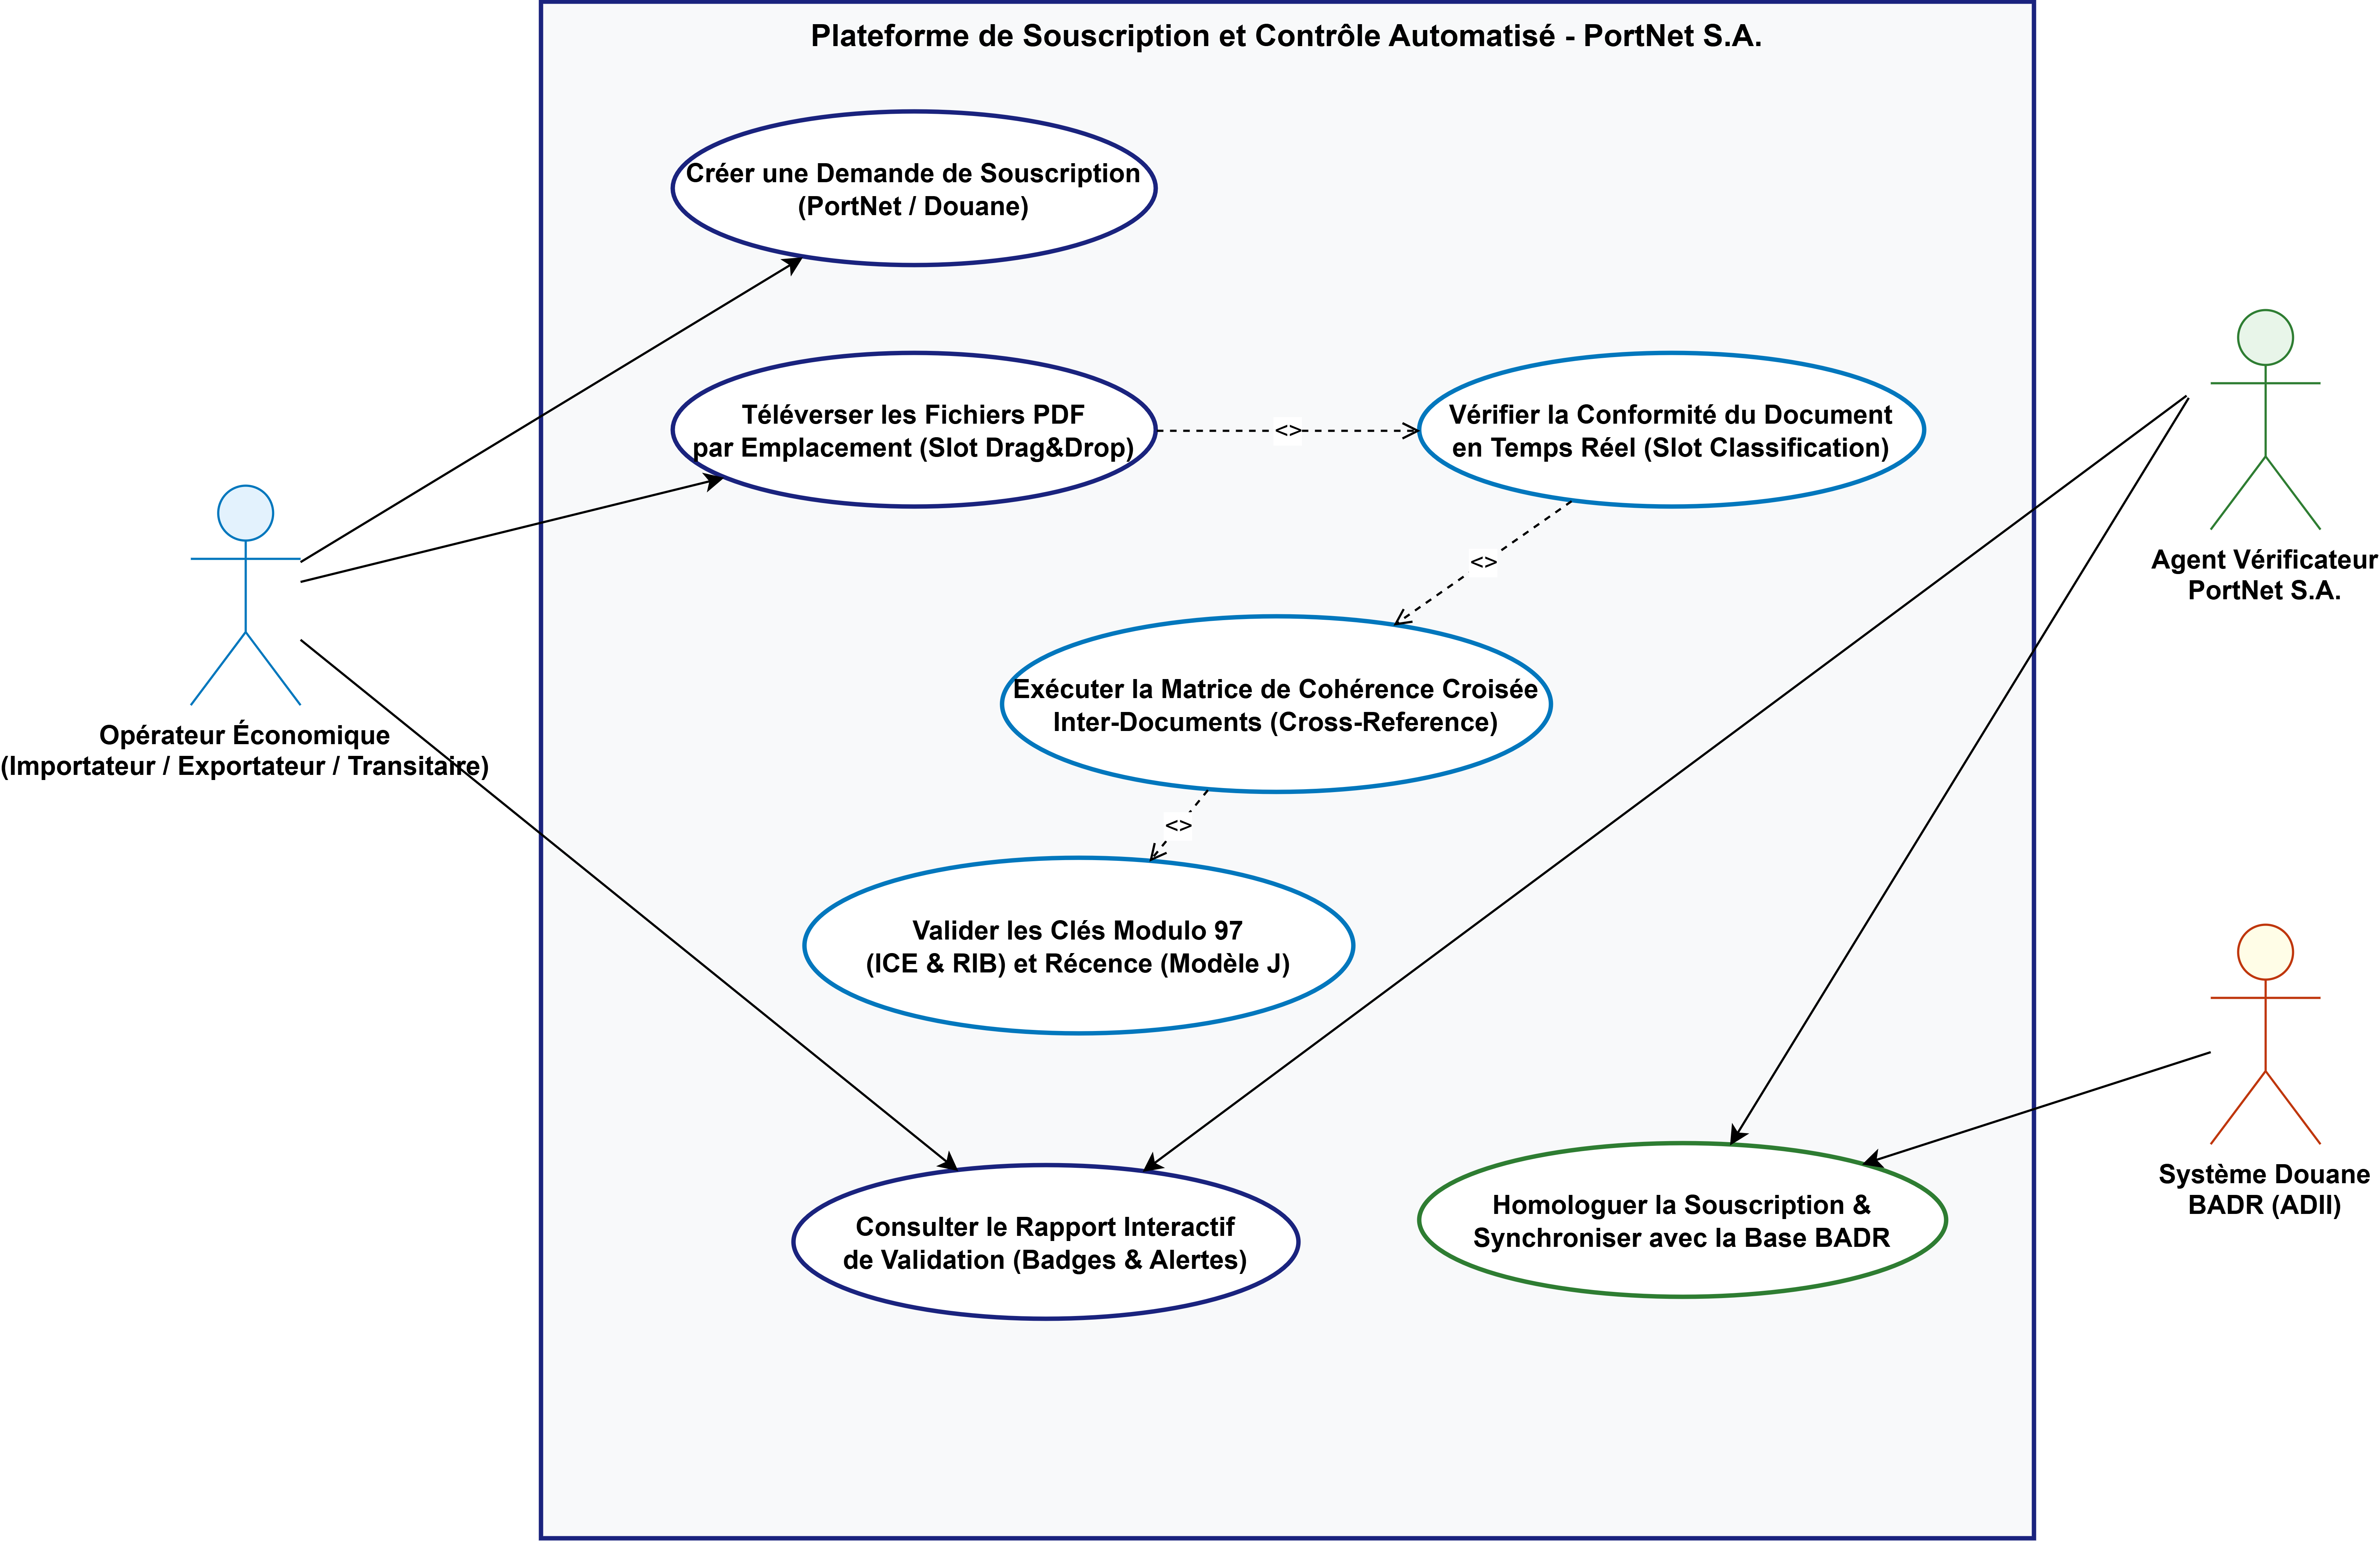
\includegraphics[width=\textwidth]{images/cas_utilisation_global.png}}{\fbox{\parbox{14cm}{\centering\vspace{3cm}\textit{Diagramme de cas d'utilisation global --- Exporter depuis cas\_utilisation\_global.drawio}\vspace{3cm}}}}
    \caption{Diagramme de cas d'utilisation global du syst\`{e}me de v\'{e}rification documentaire.}
    \label{fig:use-case-global}
\end{figure}

Les sept cas d'utilisation principaux sont :

\begin{enumerate}[leftmargin=*, itemsep=4pt]
    \item \textbf{UC-01 : Cr\'{e}er une demande de souscription} --- L'op\'{e}rateur choisit le mode (PortNet/Douane ou Douane seule) et remplit le formulaire d'inscription multi-\'{e}tapes ;
    \item \textbf{UC-02 : T\'{e}l\'{e}verser les fichiers PDF par emplacement} --- L'op\'{e}rateur d\'{e}pose chaque document dans son emplacement d\'{e}di\'{e} via Drag \& Drop ;
    \item \textbf{UC-03 : V\'{e}rifier la conformit\'{e} en temps r\'{e}el} --- Le syst\`{e}me classifie et v\'{e}rifie chaque document d\`{e}s son upload (\guillemotleft include \guillemotright{} UC-02) ;
    \item \textbf{UC-04 : Ex\'{e}cuter la matrice de coh\'{e}rence crois\'{e}e} --- Le syst\`{e}me cross-r\'{e}f\'{e}rence toutes les variables entre documents ;
    \item \textbf{UC-05 : Valider les cl\'{e}s Modulo~97} --- Le syst\`{e}me contr\^{o}le les checksums ICE et RIB ;
    \item \textbf{UC-06 : Consulter le rapport de validation} --- L'op\'{e}rateur et l'agent consultent les r\'{e}sultats avec badges visuels ;
    \item \textbf{UC-07 : Homologuer et synchroniser avec BADR} --- L'agent valide le dossier et le transmet au syst\`{e}me douanier.
\end{enumerate}

\subsection{Descriptions Textuelles des Cas d'Utilisation}

\begin{table}[H]
\centering
\small
\begin{tabularx}{\textwidth}{@{}>{\bfseries}p{3.5cm} Y@{}}
\toprule
\rowcolor{lightblue}
\'{E}l\'{e}ment & Description \\
\midrule
Cas d'utilisation & UC-03 : V\'{e}rifier la conformit\'{e} du document en temps r\'{e}el \\
Acteur principal & Syst\`{e}me (d\'{e}clench\'{e} automatiquement apr\`{e}s UC-02) \\
Pr\'{e}conditions & Un fichier PDF a \'{e}t\'{e} d\'{e}pos\'{e} dans un emplacement (slot) \\
Sc\'{e}nario principal & 1. Extraire le texte brut (Tier~1: PyMuPDF) \newline 2. Si texte $<$ 20 caract\`{e}res, repli OCR (Tier~2: Tesseract) \newline 3. Classifier le document (ancres positives + exclusions n\'{e}gatives) \newline 4. Si le type d\'{e}tect\'{e} ne correspond pas \`{a} l'emplacement, rejeter \newline 5. Parser les entit\'{e}s m\'{e}tier via l'extracteur d\'{e}di\'{e} \newline 6. Appliquer les validations locales (checksums, r\'{e}cence) \\
Postconditions & Le document est annot\'{e} (VALID / WARNING / INVALID) avec un rapport d\'{e}taill\'{e} \\
\bottomrule
\end{tabularx}
\caption{Description textuelle du cas d'utilisation UC-03.}
\label{tab:uc03-description}
\end{table}

\section{Diagrammes de S\'{e}quence}

\subsection{S\'{e}quence de V\'{e}rification d'un Document}

La figure~\ref{fig:sequence-verification} d\'{e}taille le flux de messages lors de la v\'{e}rification d'un document :

\begin{figure}[H]
    \centering
    \IfFileExists{images/diagramme_sequence_verification.png}{\includegraphics[width=\textwidth]{images/diagramme_sequence_verification.png}}{\fbox{\parbox{14cm}{\centering\vspace{3cm}\textit{Diagramme de s\'{e}quence --- V\'{e}rification d'un document --- Exporter depuis diagramme\_sequence\_verification.drawio}\vspace{3cm}}}}
    \caption{Diagramme de s\'{e}quence du processus de v\'{e}rification d'un document PDF.}
    \label{fig:sequence-verification}
\end{figure}

Le flux de messages suit la s\'{e}quence suivante :
\begin{enumerate}[leftmargin=*, itemsep=2pt]
    \item L'\textbf{Op\'{e}rateur} d\'{e}pose un fichier PDF dans un emplacement du frontend ;
    \item Le \textbf{Frontend} envoie le fichier au \textbf{Backend} via une requ\^{e}te \texttt{POST /api/verify} ;
    \item Le \textbf{Backend} invoque le \textbf{TextExtractor} (PyMuPDF) ;
    \item Si le texte est insuffisant, le \textbf{OCRExtractor} (Tesseract) prend le relais ;
    \item Le \textbf{Classifier} re\c{c}oit le texte brut et retourne le type d\'{e}tect\'{e} ;
    \item L'\textbf{Extracteur d\'{e}di\'{e}} parse les entit\'{e}s m\'{e}tier ;
    \item Les \textbf{Validators} (checksum, r\'{e}cence, format) produisent les r\'{e}sultats de validation ;
    \item Le \textbf{Backend} retourne le rapport au \textbf{Frontend} ;
    \item Le \textbf{Frontend} affiche les badges d'\'{e}tat (vert/orange/rouge).
\end{enumerate}

\subsection{S\'{e}quence d'Homologation du Dossier}

\begin{figure}[H]
    \centering
    \IfFileExists{images/diagramme_sequence_homologation.png}{\includegraphics[width=\textwidth]{images/diagramme_sequence_homologation.png}}{\fbox{\parbox{14cm}{\centering\vspace{3cm}\textit{Diagramme de s\'{e}quence --- Homologation du dossier --- Exporter depuis diagramme\_sequence\_homologation.drawio}\vspace{3cm}}}}
    \caption{Diagramme de s\'{e}quence du processus d'homologation et de synchronisation BADR.}
    \label{fig:sequence-homologation}
\end{figure}

\section{Diagramme d'Activit\'{e}}

Le diagramme d'activit\'{e} de la figure~\ref{fig:activite-traitement} mod\'{e}lise l'enchaînement complet du traitement d'un dossier de souscription \`{a} l'aide de trois couloirs (\textit{swimlanes}) : Op\'{e}rateur, Syst\`{e}me de V\'{e}rification et Agent PortNet.

\begin{figure}[H]
    \centering
    \IfFileExists{images/diagramme_activite_traitement.png}{\includegraphics[width=\textwidth]{images/diagramme_activite_traitement.png}}{\fbox{\parbox{14cm}{\centering\vspace{3cm}\textit{Diagramme d'activit\'{e} --- Traitement du dossier --- Exporter depuis diagramme\_activite\_traitement.drawio}\vspace{3cm}}}}
    \caption{Diagramme d'activit\'{e} du traitement complet d'un dossier de souscription.}
    \label{fig:activite-traitement}
\end{figure}

Les principales activit\'{e}s mod\'{e}lis\'{e}es sont :
\begin{itemize}[leftmargin=*, itemsep=2pt]
    \item \textbf{Couloir Op\'{e}rateur} : s\'{e}lection de l'organisme, remplissage du formulaire, upload des documents, consultation du rapport ;
    \item \textbf{Couloir Syst\`{e}me} : extraction PDF, classification, parsing, validation locale, cross-r\'{e}f\'{e}rence, g\'{e}n\'{e}ration du rapport ;
    \item \textbf{Couloir Agent} : consultation du rapport automatis\'{e}, d\'{e}cision d'homologation, synchronisation BADR.
\end{itemize}

\section{Diagramme d'\'{E}tats du Dossier}

Le diagramme d'\'{e}tats de la figure~\ref{fig:etat-dossier} mod\'{e}lise le cycle de vie d'un dossier de souscription :

\begin{figure}[H]
    \centering
    \IfFileExists{images/etat_dossier.png}{\includegraphics[width=\textwidth]{images/etat_dossier.png}}{\fbox{\parbox{14cm}{\centering\vspace{2.5cm}\textit{Diagramme d'\'{e}tats --- Cycle de vie du dossier --- Exporter depuis etat\_dossier.drawio}\vspace{2.5cm}}}}
    \caption{Diagramme d'\'{e}tats du cycle de vie d'un dossier de souscription.}
    \label{fig:etat-dossier}
\end{figure}

Les \'{e}tats identifi\'{e}s sont :
\begin{enumerate}[leftmargin=*, itemsep=2pt]
    \item \textbf{BROUILLON} : l'op\'{e}rateur a commenc\'{e} le formulaire mais n'a pas encore soumis ;
    \item \textbf{SOUMIS} : le formulaire et les documents ont \'{e}t\'{e} transmis au syst\`{e}me ;
    \item \textbf{EN\_V\'{E}RIFICATION} : le pipeline de validation est en cours d'ex\'{e}cution ;
    \item \textbf{EN\_ATTENTE} : le dossier est en attente de d\'{e}cision de l'agent v\'{e}rificateur ;
    \item \textbf{VALID\'{E}} : le dossier a pass\'{e} toutes les validations et a \'{e}t\'{e} approuv\'{e} ;
    \item \textbf{REJET\'{E}} : le dossier pr\'{e}sente des incoh\'{e}rences critiques n\'{e}cessitant une correction ;
    \item \textbf{SYNCHRONIS\'{E}} : le dossier valid\'{e} a \'{e}t\'{e} transmis au syst\`{e}me BADR.
\end{enumerate}

\section{Architecture \`{a} Deux Couches}

L'architecture du syst\`{e}me est organis\'{e}e en deux couches principales, illustr\'{e}es dans la figure~\ref{fig:architecture-2-couches} :

\begin{figure}[H]
    \centering
    \IfFileExists{images/architecture_2_couches.png}{\includegraphics[width=\textwidth]{images/architecture_2_couches.png}}{\fbox{\parbox{14cm}{\centering\vspace{3cm}\textit{Architecture \`{a} deux couches --- Exporter depuis architecture\_2\_couches.drawio}\vspace{3cm}}}}
    \caption{Architecture g\'{e}n\'{e}rale \`{a} deux couches du syst\`{e}me de v\'{e}rification documentaire.}
    \label{fig:architecture-2-couches}
\end{figure}

\subsection{Couche Pr\'{e}sentation (Frontend SPA)}

Le frontend est une application mono-page (SPA) en HTML, CSS et JavaScript natif. Il comprend :
\begin{itemize}[leftmargin=*, itemsep=2pt]
    \item Un \'{e}cran d'authentification (\textit{login/register}) ;
    \item Un formulaire multi-\'{e}tapes (\textit{wizard}) avec navigation par onglets ;
    \item Des zones de d\'{e}p\^{o}t (\textit{drag \& drop}) pour chaque emplacement de document ;
    \item Un rapport de validation interactif avec badges color\'{e}s (vert/orange/rouge) ;
    \item Une sidebar de navigation contextuelle.
\end{itemize}

\subsection{Couche M\'{e}tier et Donn\'{e}es (Backend FastAPI)}

Le backend expose une API REST via FastAPI et comprend :
\begin{itemize}[leftmargin=*, itemsep=2pt]
    \item \textbf{Endpoint \texttt{POST /api/inscriptions}} : r\'{e}ception du formulaire et persistance PostgreSQL ;
    \item \textbf{Endpoint \texttt{GET /api/inscriptions}} : consultation des dossiers enregistr\'{e}s ;
    \item \textbf{Module Pipeline} : orchestration du flux extraction $\to$ classification $\to$ parsing $\to$ validation ;
    \item \textbf{Module Extractors} : 7 parsers d\'{e}di\'{e}s + extracteur de texte + OCR ;
    \item \textbf{Module Validators} : checksums, r\'{e}cence, format, cross-r\'{e}f\'{e}rence.
\end{itemize}

\section{Conception de la Matrice de Coh\'{e}rence Crois\'{e}e}

La matrice de coh\'{e}rence crois\'{e}e constitue le c\oe{}ur du module de validation inter-documents. Elle op\`{e}re en comparant syst\'{e}matiquement sept variables cl\'{e}s extraites de chaque document avec les donn\'{e}es du formulaire et avec les donn\'{e}es des autres documents :

\begin{figure}[H]
    \centering
    \IfFileExists{images/matrice_coherence_croisee.png}{\includegraphics[width=\textwidth]{images/matrice_coherence_croisee.png}}{\fbox{\parbox{14cm}{\centering\vspace{2.5cm}\textit{Matrice de coh\'{e}rence crois\'{e}e --- Exporter depuis matrice\_coherence\_croisee.drawio}\vspace{2.5cm}}}}
    \caption{Conception d\'{e}taill\'{e}e de la matrice de coh\'{e}rence crois\'{e}e inter-documents.}
    \label{fig:matrice-coherence}
\end{figure}

\begin{successbox}
\textbf{R\`{e}gle de d\'{e}cision de la cross-r\'{e}f\'{e}rence} \\
Pour chaque variable partag\'{e}e : si la comparaison est strictement identique ou si le score de similarit\'{e} floue d\'{e}passe le seuil configur\'{e}, le statut est \texttt{VALID}. Si la valeur est absente dans l'un des documents, le statut est \texttt{WARNING}. Si la comparaison \'{e}choue (valeurs diff\'{e}rentes), le statut est \texttt{INVALID}. Le statut global de la cross-r\'{e}f\'{e}rence est le statut le plus s\'{e}v\`{e}re parmi toutes les comparaisons (INVALID $>$ WARNING $>$ VALID).
\end{successbox}

\section{Diagramme de Classes}

La figure~\ref{fig:classe-technique} pr\'{e}sente le diagramme de classes technique du syst\`{e}me, organis\'{e} en cinq paquetages :

\begin{figure}[H]
    \centering
    \IfFileExists{images/diagramme_classe_technique.png}{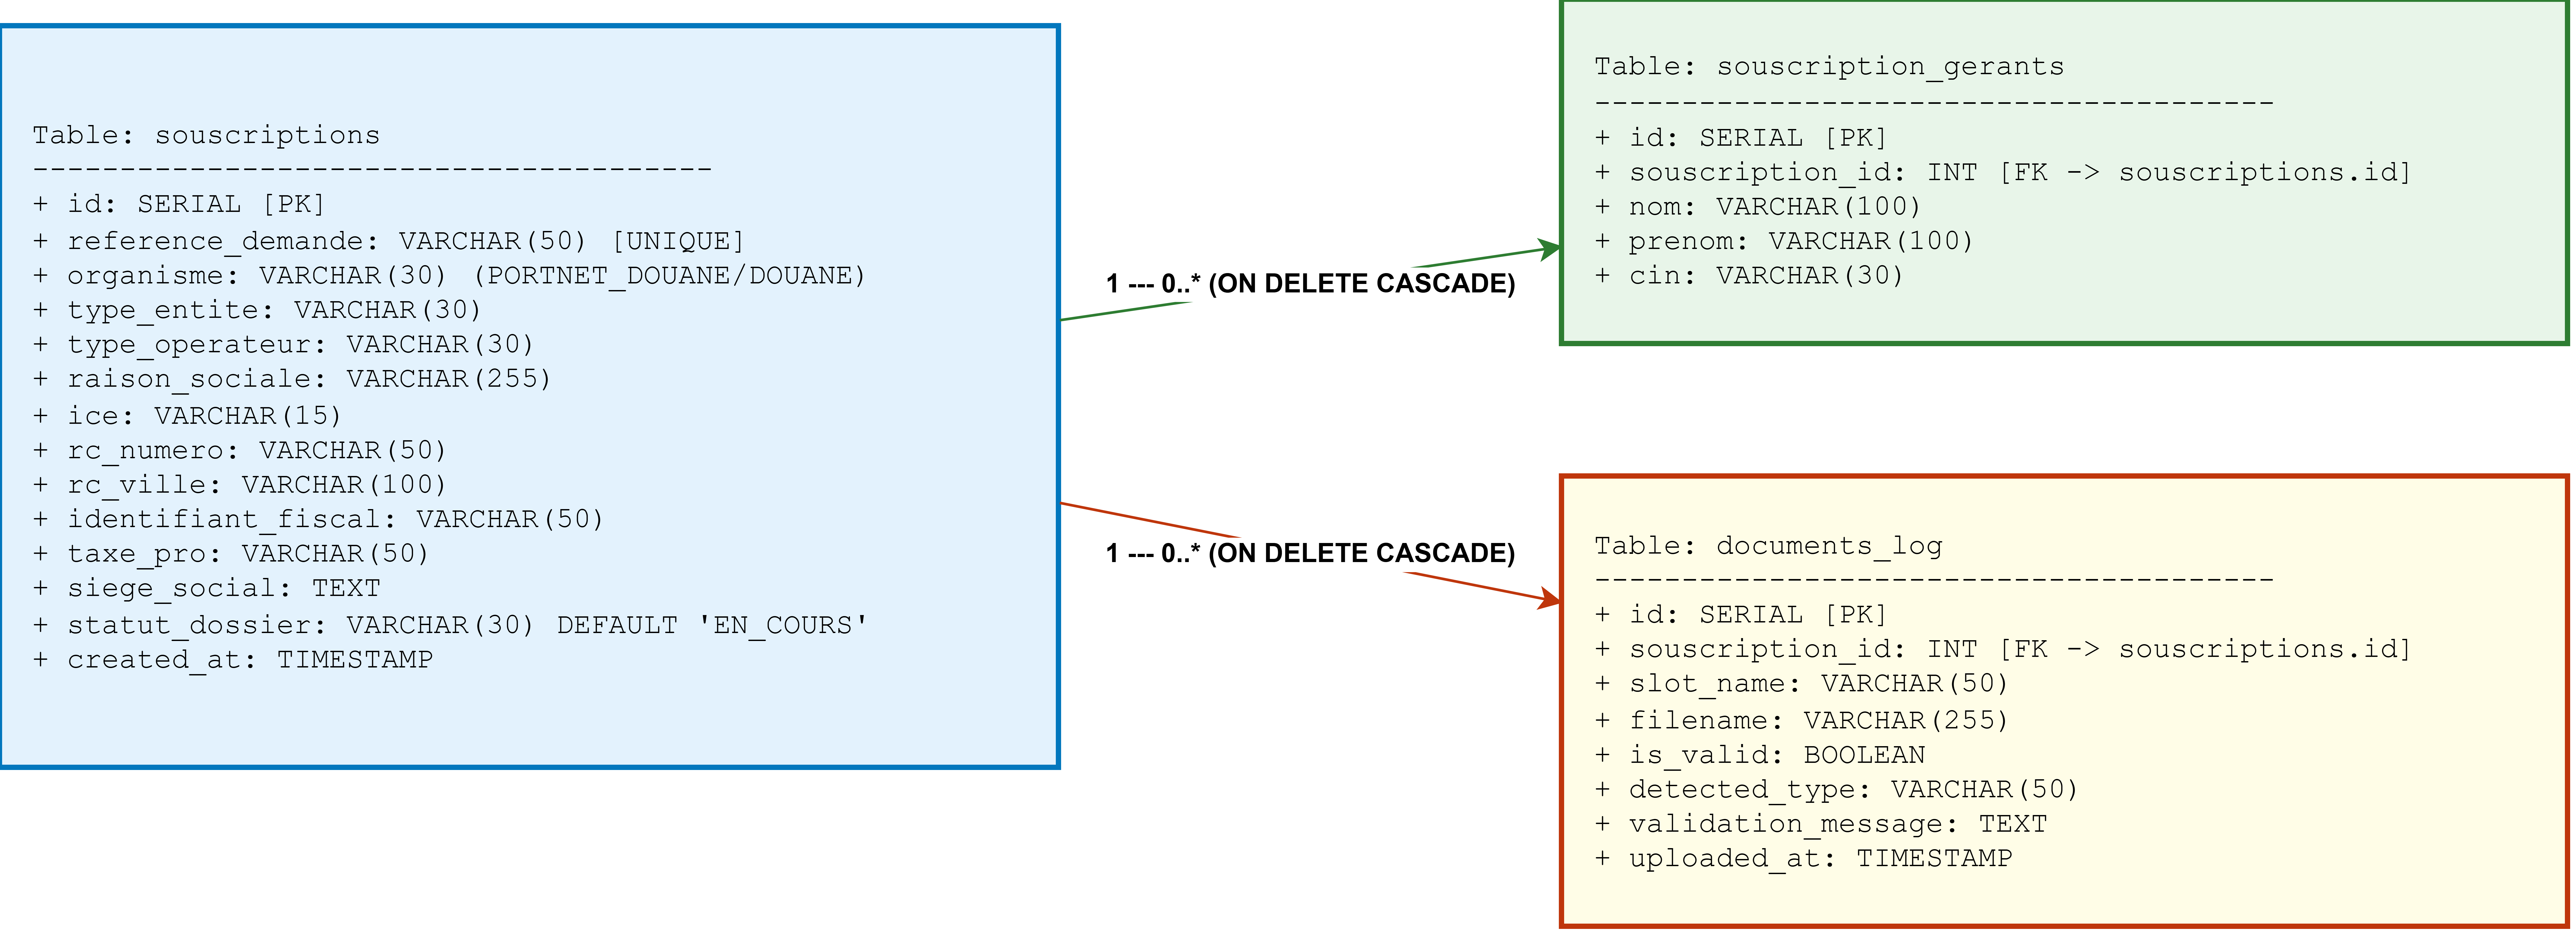
\includegraphics[width=\textwidth]{images/diagramme_classe_technique.png}}{\fbox{\parbox{14cm}{\centering\vspace{3cm}\textit{Diagramme de classes technique --- Exporter depuis diagramme\_classe\_technique.drawio}\vspace{3cm}}}}
    \caption{Diagramme de classes technique du syst\`{e}me de v\'{e}rification documentaire.}
    \label{fig:classe-technique}
\end{figure}

\begin{table}[H]
\centering
\small
\begin{tabularx}{\textwidth}{@{}>{\bfseries}p{3cm} Y@{}}
\toprule
\rowcolor{lightblue}
Paquetage & Classes principales \\
\midrule
\texttt{models} & \texttt{DocumentType}, \texttt{ValidationStatus}, \texttt{FormeJuridique}, \texttt{ExtractedDocument}, \texttt{ExtractedModelJ}, \texttt{ExtractedDocumentIF}, \texttt{ExtractedICECertificate}, \texttt{ExtractedTaxeProfessionnelle}, \texttt{ExtractedRIB}, \texttt{ExtractedDomiciliation}, \texttt{ExtractedStatuts}, \texttt{OperatorFormData}, \texttt{FieldValidation}, \texttt{FullValidationReport} \\
\texttt{extractors} & \texttt{BaseExtractor}, \texttt{TextExtractor}, \texttt{OCRExtractor}, \texttt{ModelJParser}, \texttt{DocumentIFParser}, \texttt{ICEParser}, \texttt{TPParser}, \texttt{RIBParser}, \texttt{DomiciliationParser}, \texttt{StatutsParser}, \texttt{CNIParser} \\
\texttt{validators} & \texttt{ChecksumValidator}, \texttt{RecencyValidator}, \texttt{FormatValidator}, \texttt{CrossReferenceEngine} \\
\texttt{pipeline} & \texttt{Classifier}, \texttt{Orchestrator} \\
\texttt{backend} & \texttt{FastAPIApp}, \texttt{Inscription}, \texttt{Gerant} \\
\bottomrule
\end{tabularx}
\caption{R\'{e}partition des classes par paquetage.}
\label{tab:paquetages-classes}
\end{table}

\section{Diagramme de D\'{e}ploiement}

La figure~\ref{fig:deploiement} illustre l'architecture de d\'{e}ploiement du syst\`{e}me :

\begin{figure}[H]
    \centering
    \IfFileExists{images/deploiement_infrastructure.png}{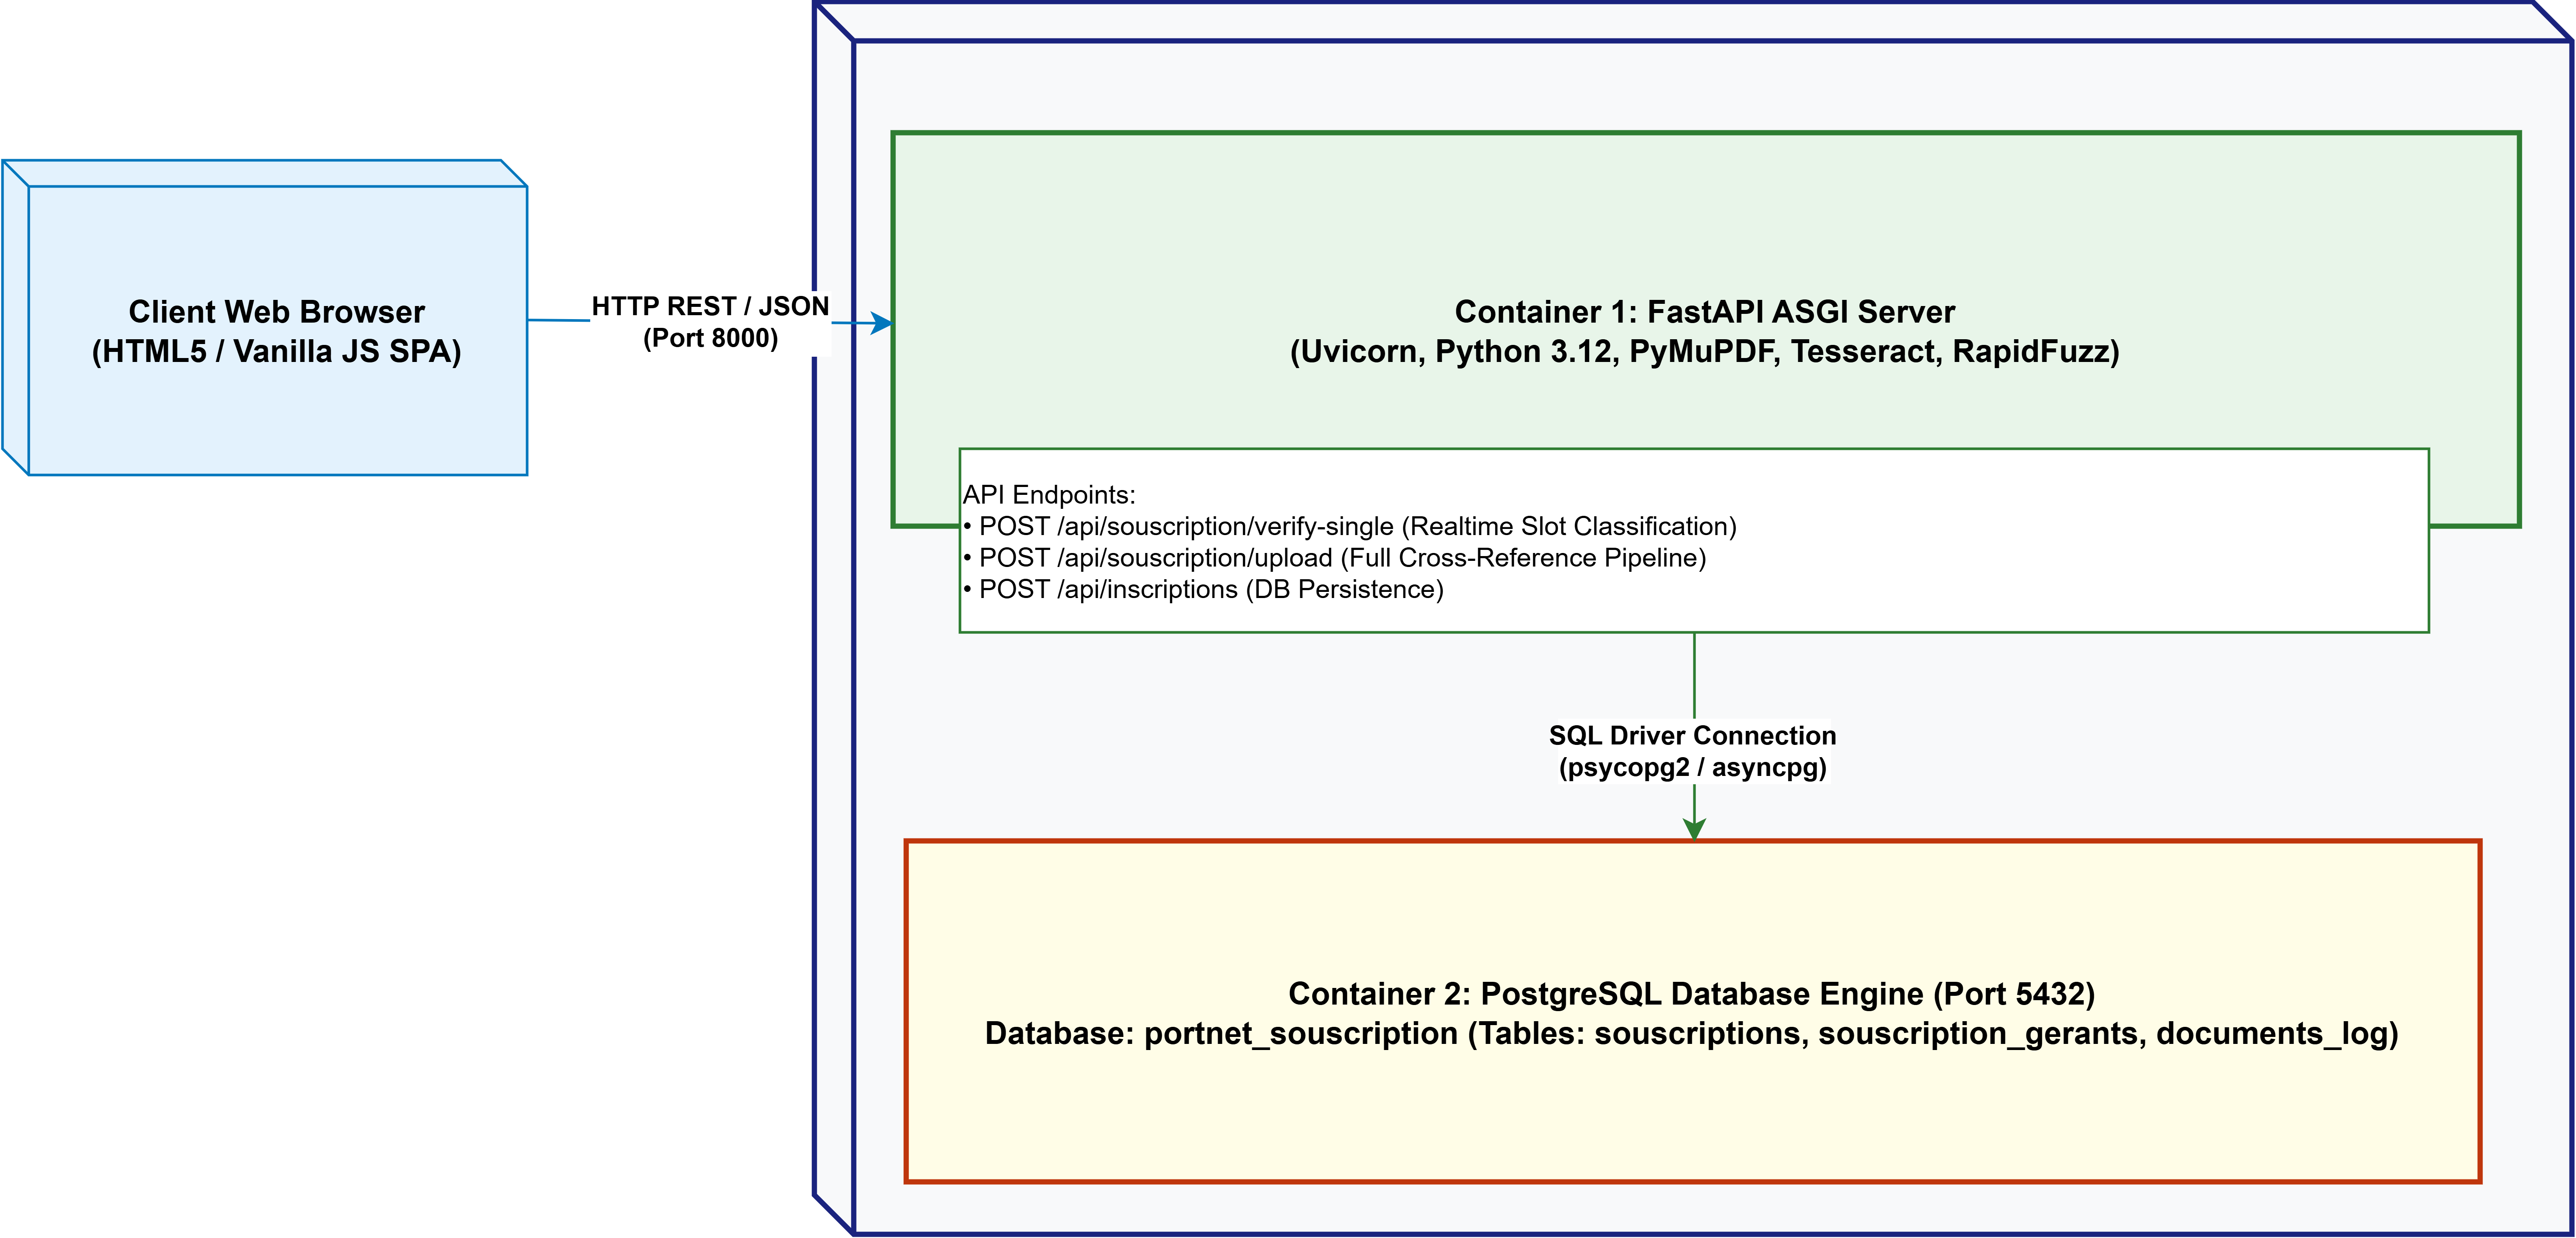
\includegraphics[width=\textwidth]{images/deploiement_infrastructure.png}}{\fbox{\parbox{14cm}{\centering\vspace{2.5cm}\textit{Diagramme de d\'{e}ploiement --- Exporter depuis deploiement\_infrastructure.drawio}\vspace{2.5cm}}}}
    \caption{Diagramme de d\'{e}ploiement de l'infrastructure du syst\`{e}me.}
    \label{fig:deploiement}
\end{figure}

\begin{table}[H]
\centering
\small
\begin{tabularx}{\textwidth}{@{}>{\bfseries}p{3cm} p{3cm} Y@{}}
\toprule
\rowcolor{lightblue}
N\oe{}ud & Composant & Technologie \\
\midrule
Navigateur Client & Frontend SPA & HTML/CSS/JS natif \\
Serveur Applicatif & Backend API & FastAPI + uvicorn \\
Conteneur Docker & Base de donn\'{e}es & PostgreSQL 15 \\
Serveur Applicatif & Pipeline Python & PyMuPDF, RapidFuzz, Pydantic \\
\bottomrule
\end{tabularx}
\caption{Correspondance n\oe{}uds, composants et technologies de d\'{e}ploiement.}
\label{tab:deploiement-noeuds}
\end{table}

\section*{Conclusion du Chapitre}

Ce chapitre a pr\'{e}sent\'{e} la conception d\'{e}taill\'{e}e du syst\`{e}me \`{a} travers neuf types de diagrammes UML. L'architecture \`{a} deux couches, le pipeline modulaire et la matrice de coh\'{e}rence crois\'{e}e constituent les fondations sur lesquelles s'appuie l'impl\'{e}mentation d\'{e}crite au Chapitre~4.
